%=========================================================================
% (c) 2011, 2012 Josef Lusticky <xlusti00@stud.fit.vutbr.cz>

\section{Algorithms}
As the figure~\ref{fig:ntp-packet} shows, there are four 64-bit long timestamps
in NTP packet: Reference, Origin, Receive and Transmit timestamp.
Using these four timestamps, NTP can compute
the offset which is given by $\theta = \frac{1}{2}[(t_1 - t_0) + (t_2 - t_1)]$,
where $t_0$ is the time of the request packet transmission,
$t_1$ is the time of the request packet reception,
$t_2$ is the time of the response packet transmission and
$t_3$ is the time of the response packet reception~\cite{ntp-algor}.

%! communication with one server

When computing result from more servers the intersection algorithms is used
for selecting the possible most exact timestamp recieved from various servers~\cite{rfc5905}.
% Derived from Murzollo algorithm but the base remains... ~\cite{ntp-history}.
The resulting exact timestamp does not have to be the same
as one of those servers provided.
First of all a set of bad and good servers must be made.
Bad servers are called Falsetickers and good are called Truechimers~\cite{rfc5905}.
The division to these sets is based on their response.
As one can assume for sensible result there must be more Truechimers than Falsetickers~\cite{rfc5905}.

Intersection algorithm computes with estimates converted to intervals.
Figure~\ref{fig:ntp-intersection} shows the computation for the following example:
If we have the estimates $10 \pm 2$, $12 \pm 1$ and $11 \pm 1$
then these intervals are $<8; 12>$, $<11; 13>$ and $<10; 12>$ which
intersect to form $<11; 12>$ or $11.5 \pm 0.5$ as consistent with all three values.
The arithmetic mean is used as a value of result.
When querying servers again, the algorithm repeats but the new result computation
also depends on the previous result~\cite{rfc5905}.
This eliminates possible jitter which can be caused by reapeatedly quering the servers
and getting slightly different answers from them.

\begin{figure}
	\centering
	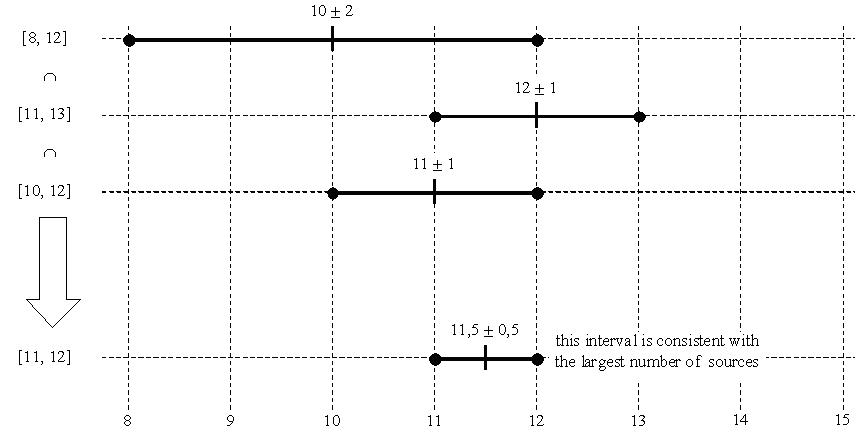
\includegraphics[width=13cm,keepaspectratio]{fig/Marzullo_example-1.jpg}
	\caption{Intersection algorithm by D. Exb}
	\label{fig:ntp-intersection}
	\bigskip
\end{figure}

%Since the clients complying with a subset of NTP, called
%the Simple Network Time Protocol (SNTPv4) [RFC4330], do not need to
%implement the mitigation algorithms ... ~\cite{rfc5905}.
